\chapter{Ringraziamenti e Roba Varia}

\graffito{L'amore non ci \'e sconosciuto...}
Yadda yadda.
\graffito{...Anche io, come voi, conosco le regole...}

\section{Ringraziamenti}

\section{SPAM: Origine di un nome}
\begin{figure}[b]
    %\centering
    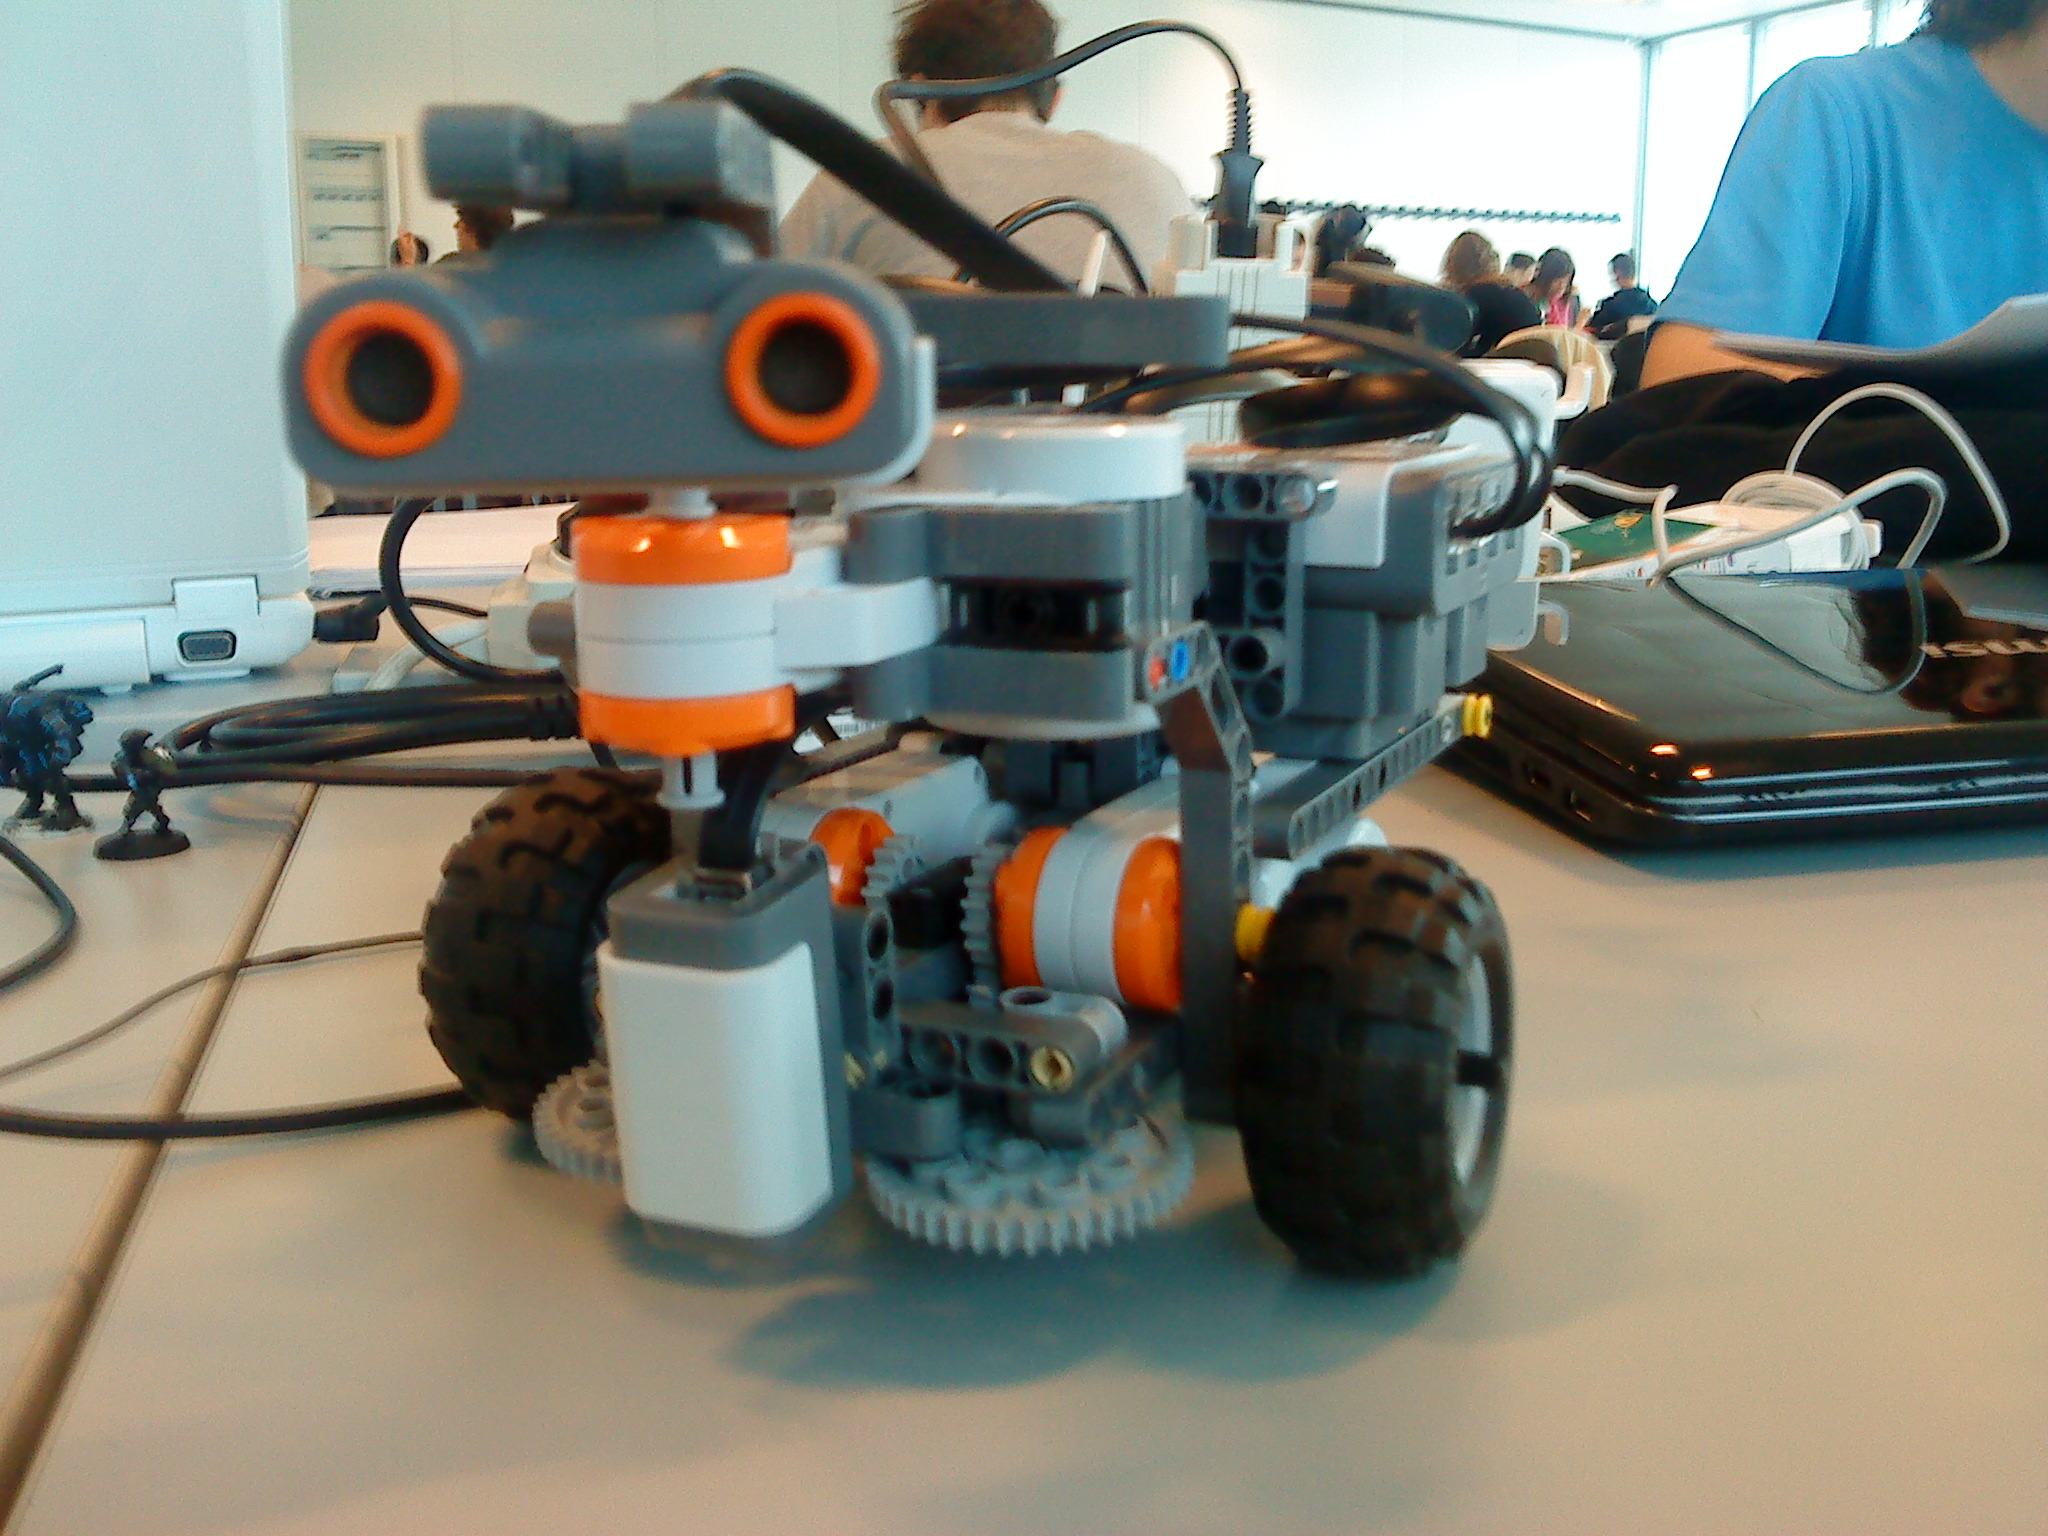
\includegraphics[width=\columnwidth]{Pictures/SPAM}
    \caption{Un'immagine dello \SPAM{} nella sua ultima versione,
    sviluppata dal Maestro Ivan ``GODS'' Simonini.}
    \label{fig:spam}
\end{figure}
In giro per il testo potrei aver utilizzato il nome \SPAM{}. Devo ammettere
che questa scelta potrebbe creare della confusione nei lettori. Ma non vi
preoccupate, ora spiegher\'o in maniera abbastanza rapida cosa significa,
che cosa \'e e tutto il resto.

\cleardoublepage
